\chapter{PENGENALAN ANTARMUKA DAN MENAMBAHKAN DATA SIG PADA APLIKASI QGIS}

Pada Bab ini kita akan mengenal bagian-bagian dasar yang biasa digunakan untuk membuat peta menggunakan QGIS 2.14, menambahkan data, dan mengeksplor data menggunakan \textit{tools-tools} yang tersedia.

\begin{enumerate}[A.]

\item \textbf{Pengenalan Antarmuka QGIS 2.14 Essen}

Bagian-bagian dari antarmuka QGIS ini seperti terlihat pada gambar \ref{fig:bagianui}.

\begin{figure}
  \centering
  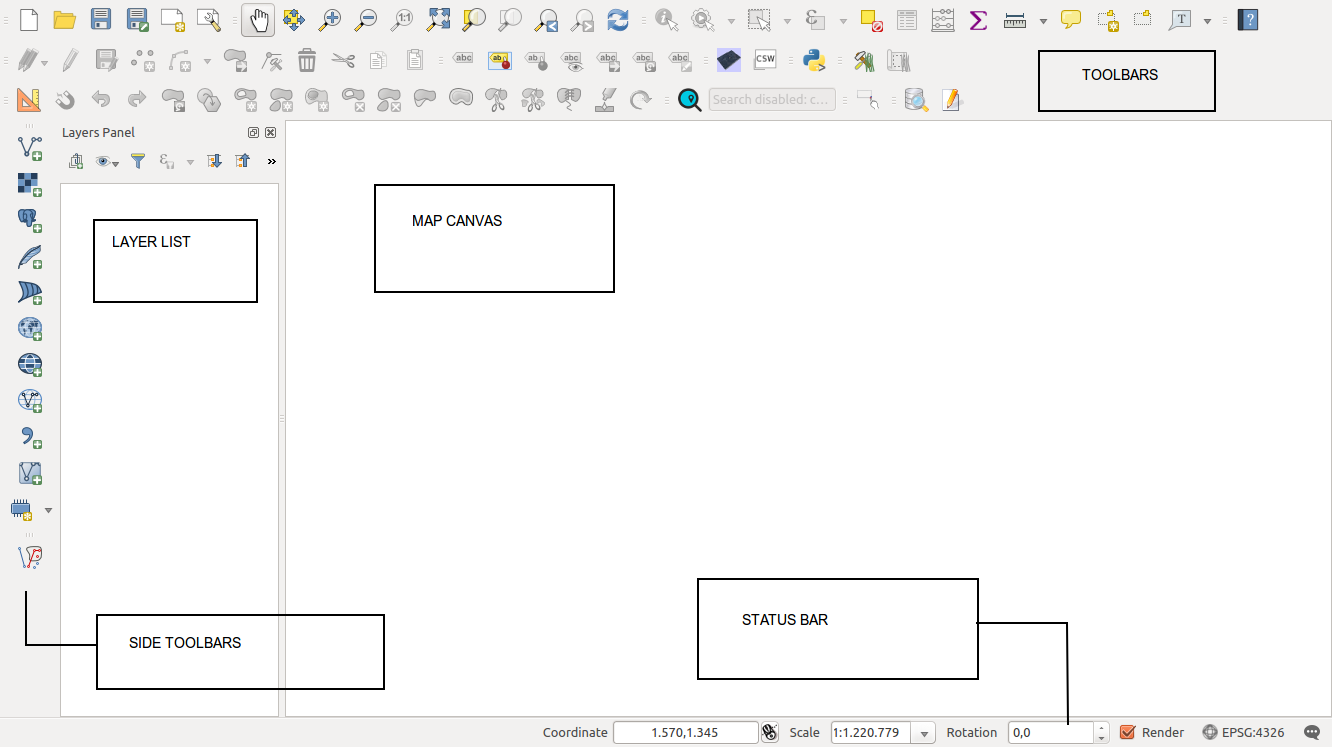
\includegraphics[width=1\textwidth]{./resources/004-bagian-qgis}
  \caption{Bagian Antarmuka QGIS}
  \label{fig:bagianui}
\end{figure}

\begin{itemize}

\item \textbf{Map Canvas}

Merupakan tempat menampilkan proyek / peta yang sedang dijalankan.

\item \textbf{Layer List}

Memuat daftar \textit{layer-layer} yang digunakan dalam proyek. Urutan \textit{layer} yang ditampilkan pada \textit{map canvas} berdasarkan urutan dari atas ke bawah pada \textit{layer list}-nya.

\item \textbf{Menu}

Bagian \textit{menu} ini tidak terlihat di gambar karena konfigurasi tampilan \textit{menu} menempel pada \textit{menu bar desktop}. \textit{Menu} ini berisi sekumpulan perintah teks untuk melakukan tugas-tugas tertentu.

\item \textbf{Toolbar dan Side Tooldbar}

Bagian ini berisi sekumpulan perintah berbasis tombol / ikon untuk melakukan tugas-tugas tertentu. \textit{Tools} dikelompokan dalam grup-grup \textit{toolbar} seperti \textit{File Toolbar}, \textit{Digitizing Toolbar}, \textit{Managed Layers Toolbar}, dan lainnya.

\item \textbf{Status Bar}

\textit{Status bar} memuat koordinat berdasarkan lokasi kursor / pointer, skala, dan sistem koordinat proyek pada \textit{map canvas}.

\end{itemize}

\item \textbf{Menambahkan Data}

Dalam QGIS dan aplikasi GIS pada umumnya, data vektor dalam format \textit{shapefile} dan data \textit{raster} yang akan ditambahkan untuk membuat sebuah \textit{project} (\texttt{*.qgis}) yang telah dibuat, melainkan hanya menyimpan \textit{style} dari data tersebut. Data tetap berada pada \textit{direktori} tempat menyimpan data, oleh karena itu satu \textit{dataset} dapat digunakan untuk berbagai \textit{project}. Berikut langkah-langkah yang dilakukan untuk menambahkan data sebagai \textit{layer} dalam QGIS.

\begin{enumerate}[1.]
  \item Klik \textit{tool} \texttt{Add Vector Layer} yang terlihat seperti pada gambar \ref{fig:addvectorlayer}.
  
\begin{figure}[H]
  \centering
  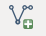
\includegraphics[scale=1]{./resources/005-ikon-add-vektor-layer}
  \caption{Ikon \textit{Add Vector Layer}}
  \label{fig:addvectorlayer}
\end{figure}

  \item Sebuah kotak dialog tempat untuk memilih \textit{file} yang akan ditambahkan ke dalam proyek QGIS akan muncul seperti pada gambar \ref{fig:addvectorlayerwindow}
  
\begin{figure}[H]
  \centering
  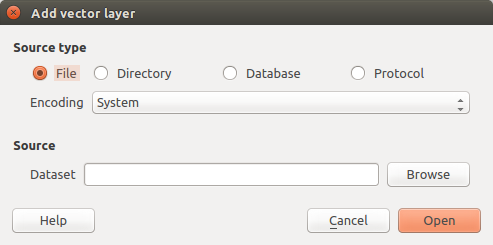
\includegraphics[scale=0.8]{./resources/006-add-vector-layer-window}
  \caption{Jendela \textit{Add Vector Layer}}
  \label{fig:addvectorlayerwindow}
\end{figure}

  \item Klik \textit{Browse} dan navigasikan pada \textit{direktori} tempat anda menyimpan \textit{shapefile}, tampilannya akan terlihat seperti gambar \ref{fig:pemilihanfilepeta}.
  
\begin{figure}[H]
  \centering
  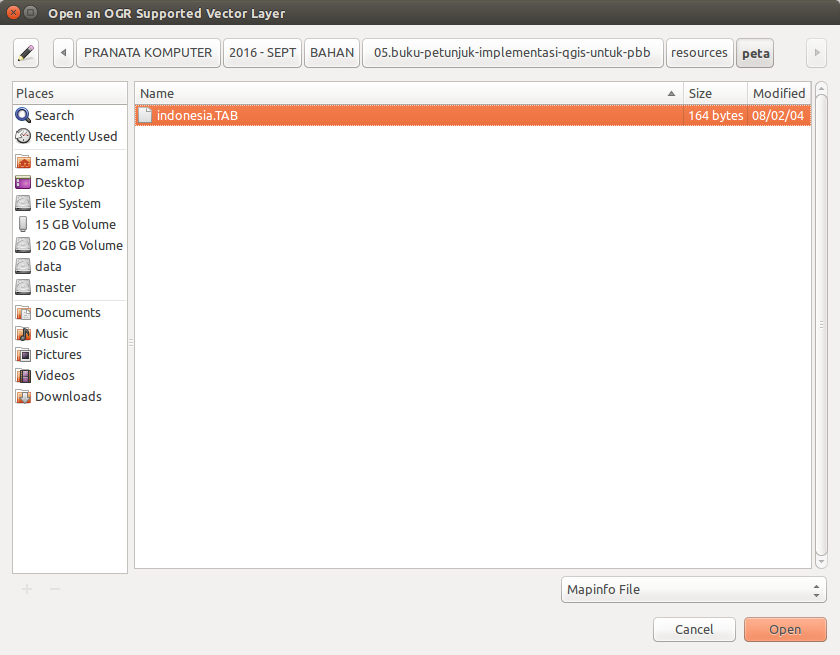
\includegraphics[width=1\textwidth]{./resources/007-pemilihan-file-peta}
  \caption{Pemilihan Layer Peta}
  \label{fig:pemilihanfilepeta}
\end{figure}

  \item Setelah memilih \textit{shapefile} yang diinginkan untuk dilihat atau diubah, klik \textit{Open} untuk memasukkan \textit{path file} ke dalam \textit{form} isian, dan klik \textit{Open} lagi pada dialog \textit{Add Vector Layer} untuk memuatnya ke dalam aplikasi. Seharusnya akan terlihat pada \textit{map canvas} seperti tampilan pada gambar \ref{fig:petaindonesiaload}
  
\begin{figure}[H]
  \centering
  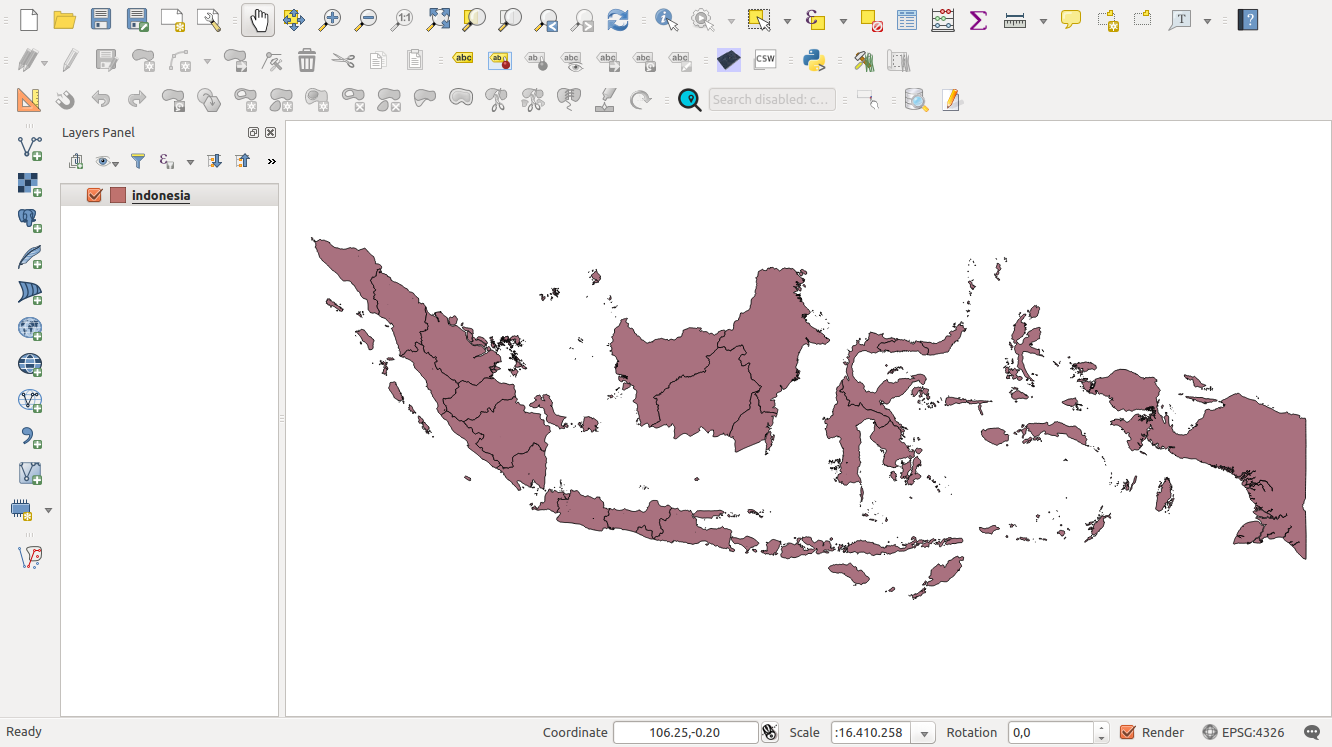
\includegraphics[width=1\textwidth]{./resources/008-peta-indonesia}
  \caption{Peta Indonesia Yang Sudah Termuat Dalam \textit{Map Canvas}}
  \label{fig:petaindonesiaload}
\end{figure}

\end{enumerate}

\item \textbf{Mengeksplor Data}

Selain menampilkan peta, \textit{layer} yang ditambahkan dapat di \textit{explore} dengan cara :

\begin{enumerate}[1.]
  \item Menavigasikan Peta
  \item Identifikasi Fitur
  \item Memeriksa Atribut
  
\end{enumerate}

\end{enumerate}